\section{Object Reconstruction and Selection}
\label{sec:object_reconstruction}

The reconstruction and selection of physics objects
% , i.e.\ objects representing the signature of particles produced in
% \pp~collisions,
is described in this section. The most relevant objects for this search are
electrons, muons, \tauhadvis, jets, $b$-tagged jets, and the missing transverse
momentum. These objects are reconstructed and identified using algorithms that
target their distinct signatures in the ATLAS detector
(cf.~\Cref{sec:object_reco_at_atlas}).
% The same algorithms are used to reconstruct and identify objects in simulation
% and in data recorded with the detector.
Differences between the performance of the object reconstruction and selection
in simulation and data are accounted for by dedicated calibration measurements
of efficiencies, energy/momentum scales and resolutions.
% Uncertainties on these measurements are propagated to the final results by
% performing variations of these properties in simulation.

The baseline selection of objects used in this search is described in the
following. More restrictive selections are applied as part of the event
selection, which is discussed in \Cref{sec:event_selection}.
\begin{description}

\item[Electrons] are required to have $\pT > \SI{7}{\GeV}$ and to be
  reconstructed within the acceptance of the tracking detectors,
  $|\eta| < \num{2.47}$. Electrons in the transition region between the barrel
  and end-cap electromagnetic calorimeters, $1.37 < |\eta| < 1.52$, are
  rejected. All reconstructed electrons have to pass the loose working point of
  a likelihood-based electron identification algorithm to reject non-prompt
  electrons and electron candidates originating from jets. This working point
  has a target identification efficiency of \SI{93}{\percent} for electrons with
  transverse momenta of about \SI{40}{\GeV}~\cite{EGAM-2018-01,PERF-2017-01}.

  % FCLoose
  % topoetcone20/pT < 0.2
  % ptvarcone20_TightTTVA_pt1000/pT < 0.15
  Electron candidates with high activity in the vicinity of the electron are
  rejected by making a loose requirement on both calorimeter- and track-based
  isolation variables~\cite{EGAM-2018-01}.
  % ($E_{\text{T}}^\text{cone20} / \pT < 0.2$ and
  % $p_{\text{T}}^{\text{varcone20}}/ \pT < 0.15$ as described in
  % Ref.~\cite{EGAM-2018-01}).
  The electron selection efficiency of the isolation requirement exceeds
  \SI{95}{\percent} for electrons with $\pT > \SI{20}{\GeV}$, quickly
  approaching efficiencies close to \SI{100}{\percent} at higher transverse
  momenta~\cite{EGAM-2018-01}. This requirement is inverted as part of the
  \faketauhadvisC background estimation in the \lephad channel to provide a
  control region (CR) enhanced in multi-jet events.
  % Energy calibration???

\item[Muons] are required to have $\pT > \SI{7}{\GeV}$ and pass the loose
  identification working point (cf.~\Cref{sec:muon_rec}). The muon
  identification efficiency of the loose working point exceeds \SI{97}{\percent}
  for muons with $\pT > \SI{10}{\GeV}$ in simulated \ttbar
  events~\cite{MUON-2018-03}. In addition, muons are required to pass the loose
  isolation working point based on isolation requirements combining information
  on charged and neutral particle signatures using a particle flow
  approach~\cite{MUON-2018-03}. The muon selection efficiency of the isolation
  working point exceeds \SI{97}{\percent} for muons with $\pT > \SI{20}{\GeV}$
  in simulated \ttbar events~\cite{MUON-2018-03}. The isolation requirement is
  inverted to provide a CR for the \faketauhadvisC background estimation in the
  \lephad channel.

  % Muons passing the loose working point are a superset of medium muons which
  % are defined according to Ref.~\cite{MUON-2018-03} as: muons passing either
  % the \emph{combined} or \emph{inside-out combined} reconstruction in
  % $|\eta| < 2.5$; muons passing either the \emph{muon-spectrometer
  % extrapolated} or \emph{silicon-associated forward} reconstruction in
  % $2.5 < |\eta| < 2.7$. Various requirements are set on the muon
  % reconstruction quality and matching between ID and MS tracks which depend on
  % the muon reconstruction type and detector region. The loose identification
  % working point additionally allows for \emph{calorimeter-tagged} and
  % \emph{segment-tagged} muons in $|\eta| < 0.1$, a region insufficiently
  % covered by the MS, to improve the muon selection efficiency.

  % isPflowLoose_VarRadIso
  % (ptvarcone30_TightTTVA_pt500 + 0.4 neflowisol20) / pT < 0.16

  % $p_{\text{T}}^{\text{varcone30}} + 0.4 \times E_{\text{T}}^{\text{neflow20}}
  % < 0.16$~\cite{MUON-2018-03}

\item[\tauhadvis] are required to have $\pT > \SI{20}{\GeV}$ and $|\eta| <
  2.5$. In addition, \tauhadvis candidates in the transition region between the
  barrel and end-cap calorimeters, $1.37 < |\eta| < 1.52$, are rejected. Only
  \tauhadvis candidates with one or three associated charged-particle tracks are
  considered. The total electric charge of these tracks is required to be
  $\pm 1$.

  A BDT-based electron veto algorithm is applied to 1-prong \tauhadvis
  candidates to reject cases where electrons are reconstructed as 1-prong
  \tauhadvis. This algorithm has an efficiency of \SI{95}{\percent} in selecting
  \tauhadvis candidates originating from hadronic \tauleptonC decays.

  The loose working point of the RNN-based \tauid algorithm introduced in
  \Cref{sec:tauid} is used to reject \tauhadvis candidates originating from
  quark- and gluon-initiated jets. This working point targets a true \tauhadvis
  selection efficiency of \SI{85}{\percent} (\SI{75}{\percent}) in simulated
  $\gamma^* \to \tauhad\tauhad$ events for 1-prong (3-prong) \tauhadvis.

  % The \tauhadvis energy calibration is performed by combining a
  % calorimeter-based energy measurement with information from the tau particle
  % flow algorithm~\cite{PERF-2014-06} in boosted regression trees.

\item[Anti-\tauhadvis] are used to define CRs for the \faketauhadvisC background
  estimation. They follow the same selection criteria as \tauhadvis except for a
  partial inversion of the \tauid requirement. Specifically, \tauhadvis
  candidates are considered to be anti-\tauhadvis if they fail the loose \tauid
  working point but pass a very loose selection on the \tauid score of
  $\text{RNN score} > 0.01$.
  % , which corresponds to a true \tauhadvis selection efficiency of about
  % \SI{99}{\percent} in simulated $\gamma^* \to \tauhad\tauhad$ events.

  Anti-\tauhadvis are only considered in events with fewer than two (one)
  \tauhadvis passing the selection criteria of the \hadhad (\lephad) channel. In
  this case, anti-\tauhadvis are randomly selected until the required number of
  (anti-)\tauhadvis candidates, two in the \hadhad and one in the \lephad
  channel, is achieved. Anti-\tauhadvis that are not selected by the random
  anti-\tauhadvis selection
  % are treated as jets and
  are removed as part of an overlap removal procedure that is discussed
  in~\Cref{sec:overlap_removal}.

  % The \hadhad and \lephad channels use the presence of anti-\tauhadvis to
  % define CRs for the estimation of backgrounds with \faketauhadvis.

\item[Jets] are reconstructed using the anti-\kt algorithm with a radius
  parameter of~$R = 0.4$. The inputs to the jet algorithm are provided by the
  particle flow reconstruction algorithm previously described
  in~\Cref{sec:jet_rec}.

  % , described in Refs.~\cite{PERF-2015-09,JETM-2018-05}, exploiting the
  % superior momentum resolution of the tracking system for charged particles
  % with low transverse momenta by replacing the calorimetric measurement of
  % their energy with a tracking-based momentum measurement, necessitating the
  % subtraction of energy deposits by charged particles in the calorimeter. The
  % particle flow algorithm provides an improved jet energy and angular
  % resolution as well as pile-up stability compared to jets constructed based
  % on topological clusters in the calorimeters (at EM scale)
  % only~\cite{PERF-2015-09,JETM-2018-05}.

  Jets in the central (forward) region of the detector defined by $|\eta| < 2.5$
  ($2.5 < |\eta| < 4.5$) are required to fulfil~$\pT > \SI{20}{\GeV}$
  ($\pT > \SI{30}{\GeV}$). Jets originating from pile-up are suppressed by
  ensuring that all jets pass Jet Vertex Tagger (JVT) requirements. In the
  central region, jets have to pass the tight JVT working
  point~\cite{PERF-2014-03}. Jets in the forward regions
  % , which lack tracking system coverage,
  are required to fulfil the loose working point of a dedicated JVT for forward
  jets~\cite{PERF-2016-06-witherratum,ATL-PHYS-PUB-2019-026}.

  A multivariate $b$-tagging algorithm is applied to all jets in the central
  region to identify jets originating from $b$~quarks.
  % , distinguishing them from jets initiated by gluons or quarks of light- or
  % charm-flavour.
  The \textsc{DL1r} algorithm~\cite{FTAG-2019-07} is used, which combines the
  scores of several low-level taggers that exploit the signature of displaced
  decays of $b$-hadrons using information on the track impact parameters
  (\textsc{IP2D}, \textsc{IP3D} \& \textsc{RNNIP}) and secondary vertices
  (\textsc{SV1} \& \textsc{JetFitter}). A $b$-tagging working point with an
  efficiency of \SI{77}{\percent} of correctly tagging $b$-jets in simulated
  \ttbar events is used.

\item[The missing transverse momentum (\pTmiss)] is reconstructed using the
  object-based definition of \pTmiss previously introduced in
  \Cref{sec:atlas_met}. The \pTmiss reconstruction uses the definitions of
  electrons, muons, \tauhadvis, and jets introduced in this section. Selected
  anti-\tauhadvis are treated as \tauhadvis in the reconstruction of the missing
  tranverse momentum.

  % In this search it is used to reconstruct the signatures of neutrinos
  % produced in decays of \tauleptons and semi-leptonic decays of hadrons.

  % An object-based definition of the missing transverse
  % momentum~\cite{PERF-2016-07} is adopted that uses reconstructed and
  % calibrated objects, i.e.\ electrons, muons, \tauhadvis, and jets as defined
  % previously after an ambiguity resolution step introduced
  % in~\Cref{sec:overlap_removal}, as inputs to the \pTmiss reconstruction. Soft
  % charged-particle radiation that is not part of any reconstructed object is
  % accounted for by the so-called track soft term. The track soft term is
  % defined as the vectorial sum of charged-particle track
  % $\myvec{p}_{\text{T}}$ over all tracks passing track quality criteria that
  % are associated to the primary vertex of the hard interaction but not any
  % reconstructed object. The object-based \pTmiss is subsequently reconstructed
  % as the negative vectorial sum of transverse momenta of calibrated objects
  % and the track soft term.

  % The vector of the missing transverse momentum in the transverse plane is
  % denoted as \pTmiss and its magnitude as \pTmissAbs, hereafter.
\end{description}


\subsection{Overlap Removal}%
\label{sec:overlap_removal}

The object reconstruction and selection described previously does not ensure
that detector signatures can be unambiguously assigned to exactly one
reconstructed object. Any ambiguities are resolved by performing an overlap
removal procedure. This procedure rejects objects that can be associated, either
geometrically or by shared charged-particle tracks, with an object of higher
priority. In the case of geometric matching, the association is performed on the
basis of the angular distance
\begin{align*}
  \dRy = \sqrt{\Delta y^2 + \Delta \phi^2} \,\text{,}
\end{align*}
where $\Delta y$ and $\Delta \phi$ refers to the differences in rapidity and
azimuthal angle of two objects, respectively.

A sequential procedure is used to resolve the overlaps of reconstructed physics
objects. The procedure is summarised in~\Cref{tab:overlap_removal} following
recommendations developed by the ATLAS collaboration. The last three steps serve
to resolve overlaps between jets and anti-\tauhadvis. This procedure establishes
the following priority between jets, \tauhadvis, and selected anti-\tauhadvis:
\begin{center}
  \tauhadvis > \btagged jet > anti-\tauhadvis > untagged jet.
\end{center}
An alternative priority given by
\begin{center}
  \btagged jet > \tauhadvis > anti-\tauhadvis > untagged jet
\end{center}
was also considered but found to reduce the signal acceptance when selecting
events with 2 \btagged jets due to the limited \tauhadvis rejection of the
\textsc{DL1r} \btag algorithm at the \SI{77}{\percent} efficiency working
point. The alternative leads to a relative reduction in SM \HH signal acceptance
by \SI{13}{\percent} (\SI{8}{\percent}) in the \hadhad (\lephad)
channels. Therefore, \tauhadvis take precedence over $b$-tagged jets in the
overlap removal procedure as a means to maximise the signal acceptance.

\begin{table}[htbp]
  \centering

  % https://gitlab.cern.ch/atlas/athena/tree/21.2/PhysicsAnalysis/AnalysisCommon/AssociationUtils/
  % Harmonization note: https://cds.cern.ch/record/1743654/files/ATL-COM-PHYS-2014-451.pdf

  \caption[Summary of the sequential overlap removal algorithm.]{Summary of the
    sequential overlap removal algorithm with rows representing steps of the
    procedure. Steps are executed from top to bottom, rejecting objects in the
    ``Reject'' column in favour of objects in the ``Accept'' column if the
    condition is fulfilled.}%
  \label{tab:overlap_removal}

  \resizebox{\textwidth}{!}{%
    \begin{tabular}{lll}
  \toprule
  Reject & Accept & Condition \\
  \midrule

  % https://gitlab.cern.ch/atlas/athena/-/blob/21.2/PhysicsAnalysis/AnalysisCommon/AssociationUtils/Root/EleEleOverlapTool.cxx
  $e_1$ & $e_2$ & $e_1$ and $e_2$ share the charged particle track and $\pT(e_1) < \pT(e_2)$. \\[0.5em]

  % https://gitlab.cern.ch/atlas/athena/-/blob/21.2/PhysicsAnalysis/AnalysisCommon/AssociationUtils/Root/TauLooseEleOverlapTool.cxx
  \tauhadvis & $e$ & $\dRy < 0.2$ and $e$ passes the loose likelihood-based electron identification. \\[0.5em]

  % https://gitlab.cern.ch/atlas/athena/-/blob/21.2/PhysicsAnalysis/AnalysisCommon/AssociationUtils/Root/TauLooseMuOverlapTool.cxx
  \tauhadvis & $\mu$ & $\dRy < 0.2$ and either: \\
         && \hspace{0.5em}-\, \tauhadvis $\pT \leq \SI{50}{\GeV}$: $\pT(\mu) > \SI{2}{\GeV}$ \\
         && \hspace{0.5em}-\, \tauhadvis $\pT > \SI{50}{\GeV}$: $\pT(\mu) > \SI{2}{\GeV}$ and $\mu$ passes combined muon reconstruction. \\[0.5em]

  % https://gitlab.cern.ch/atlas/athena/-/blob/21.2/PhysicsAnalysis/AnalysisCommon/AssociationUtils/Root/EleMuSharedTrkOverlapTool.cxx
  $\mu$ & $e$ & $\mu$ is calorimeter-tagged and shares inner detector track with $e$. \\[0.5em]
  $e$   & $\mu$ & Both share the inner detector track. \\[0.5em]

  % Note: We do not use heavy flavour aware OLR

  % https://gitlab.cern.ch/atlas/athena/-/blob/21.2/PhysicsAnalysis/AnalysisCommon/AssociationUtils/Root/EleJetOverlapTool.cxx
  jet   & $e$ & $\dRy < 0.2$ \\[0.5em]
  $e$   & jet & $\dRy < 0.4$ \\[0.5em]

  % https://gitlab.cern.ch/atlas/athena/-/blob/21.2/PhysicsAnalysis/AnalysisCommon/AssociationUtils/Root/MuJetOverlapTool.cxx
  jet   & $\mu$ & The ID track of the muon is ghost-associated$^\dagger$ to the jet and the jet has fewer than three \\
         && ghost-associated ID tracks with $\pT > \SI{500}{\MeV}$. \\[0.5em]
         % && \hspace{0.5em}-\, The jet has fewer than three ghost-associated ID tracks with $\pT > \SI{500}{\MeV}$ \\
         % && \hspace{0.5em}-\, $\pT(\mu) / \pT(\text{jet}) > 0.5$ and $\pT(\mu) / \sum \pT(\text{track}) > 0.7$, where the sum goes over \\

  $\mu$ & jet & $\dRy < 0.4$ \\

  %jet - 𝜇: Reject jet if 𝑁track < 3 (𝑝 T, track > 500 MeV), and Δ𝑅 𝑦 < 0.2

  \midrule
  jet & \tauhadvis & ... \\[0.5em]
  anti-\tauhadvis & jet & ... \\[0.5em]
  jet & anti-\tauhadvis & ... \\
  \bottomrule
\end{tabular}

%%% Local Variables:
%%% mode: latex
%%% TeX-master: "../phd_thesis"
%%% End:

  }
\end{table}

% Due to a bug in the PFlow jet reconstruction, an additional OLR step removing
% prompt muons being reconstructed as fake jets is implemented in the official
% ASG OLR tool.

\subsection{$H \to \bbbar$ Candidate Reconstruction}%
\label{sec:hbb_reco}%
\label{sec:bjet_momentum_corrections}

The $H \to \bbbar$ candidate is reconstructed using jets in the central region
of the detector. In events with two \btagged jets, the four-momentum of the
Higgs boson candidate is reconstructed by summing the four-momenta of both
\btagged jets. In regions with fewer than two \btagged jets, which are used as
control and validation regions, the Higgs candidate four-momentum is
reconstructed as the sum of four-momenta of either the \btagged jet and the
\pT-leading untagged jet (1 $b$-tag regions) or the sum of the two \pT-leading
untagged jets (0 $b$-tag regions). Regions with more than two \btagged jets are
not considered in this search. The reconstructed Higgs boson candidate is used
to calculate the invariant mass of the $\bbbar$-system, \mBB, which is an
important variable in distinguishing signal from background events.

Corrections are applied to $b$-tagged jets in order to improve the scale and
resolution of the $b$-jet momentum reconstruction.
% , consequently improving the scale and resolution of the reconstructed \mBB.
These corrections are applied in addition to the standard jet
calibration~\cite{JETM-2018-05}, targeting the effects of out-of-cone radiation
and semi-muonic $b$- or $c$-hadron decays inside the $b$-jet on the
four-momentum of reconstructed jets. Two separate corrections, which were
previously used by the ATLAS collaboration in
Refs.~\cite{HIGG-2016-29,HIGG-2018-04,HIGG-2018-51}, are applied:
\begin{description}

\item[Muon-in-jet correction] Muons produced in decays of $b$- or $c$-hadrons
  inside $b$-jets deposit little energy in the calorimeters, thus leading to an
  underestimation of the jet four-momentum. The muon-in-jet correction is
  applied when a muon with $\pT > \SI{4}{\GeV}$ passing the \emph{medium}
  selection working point can be found within a variable size cone centred on
  the jet axis.
  % (i.e.\ a shrinking cone with increasing \pT of the muon).
  No requirements are applied on the isolation of muons entering the muon-in-jet
  correction. In case one or more muons fulfil the criteria, the muon closest to
  the jet axis is selected. The four-momentum of the selected muon is added to
  the four-momentum of the jet, after correcting for the energy it deposited in
  the calorimeters.

\item[\pTreco correction] The \pTreco correction accounts for out-of-cone
  radiation as well as momentum carried away by neutrinos produced in
  semi-leptonic decays of hadrons in the jet. It is derived using $b$-tagged
  jets in simulated \ttbar events as a function of the \pT of the reconstructed
  jet, \pTreco, separately for jets containing a muon (according to the criteria
  of the muon-in-jet correction) and jets that do not contain a muon. The
  correction is applied as a multiplicative factor on the jet momentum scale and
  is derived as the ratio $p_{\text{T}}^{\text{truth}} / \pTreco$ in bins of
  \pTreco, where $p_{\text{T}}^{\text{truth}}$ is the transverse momentum of the
  truth jet, a jet constructed from generator-level particles, that is
  geometrically matched to the jet at reconstruction-level.

\end{description}
Both corrections are performed at the level of individual jets and do not use
information about the remainder of the event.

The effect of these corrections on the reconstructed \mBB in simulated SM \HH
events in the \hadhad channel is depicted
in~\Cref{fig:bjet_momentum_corr_mbb}. The improvement in the $b$-jet momentum
scale and resolution from the muon-in-jet correction and the \pTreco correction
lead to a relative reduction of the width of the Higgs boson mass peak in the
\mBB distribution of about \SI{13}{\percent} as measured by the full width at
half maximum.

\begin{figure}[htbp]
  \centering

  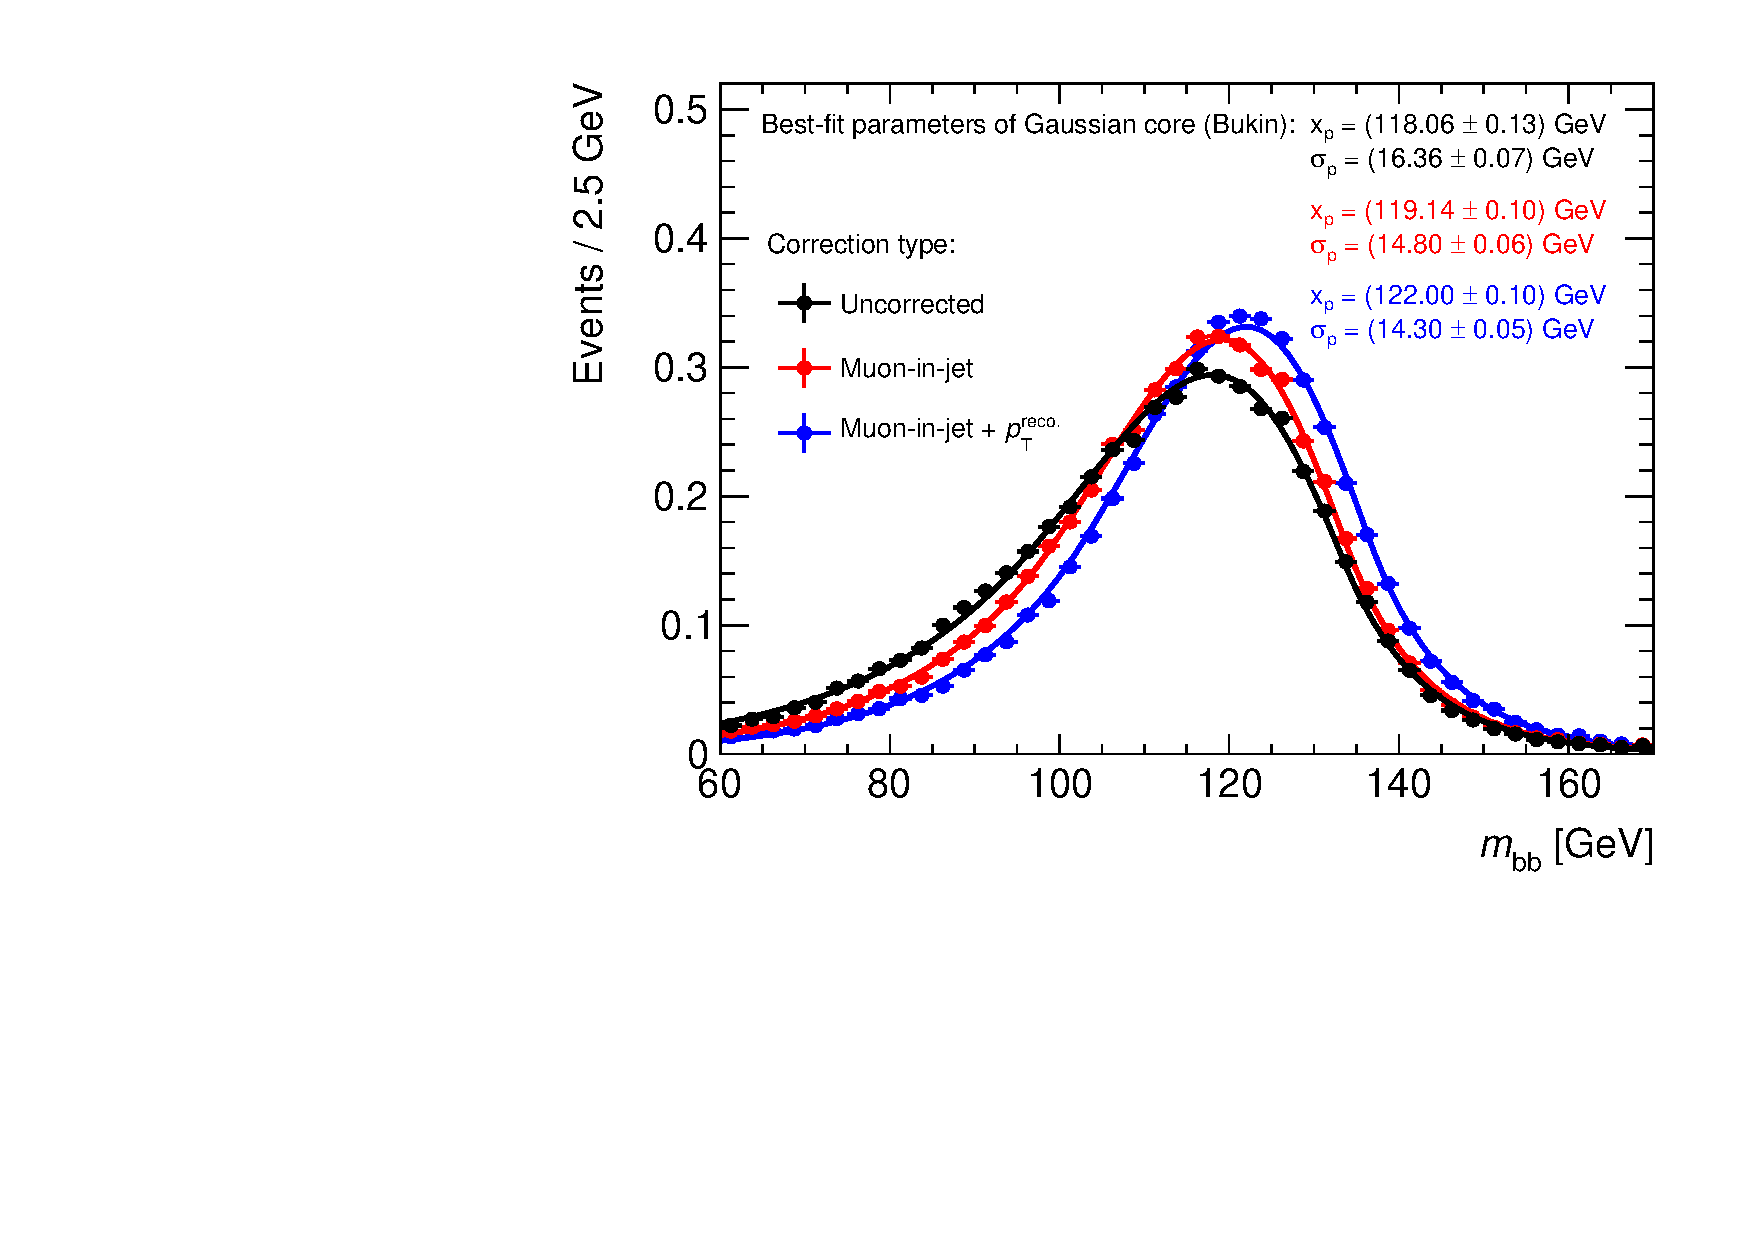
\includegraphics[width=0.6\textwidth]{reconstruction/bjet_corrections}

  \caption[The effect of $b$-jet momentum corrections on the reconstructed \mBB
  in simulated SM~\HH events in the 2~$b$-tag region of the \hadhad
  channel.]{The effect of $b$-jet momentum corrections on the reconstructed \mBB
    in simulated SM \HH events in the 2~$b$-tag region of the \hadhad
    channel. Bukin functions~\cite{Bukin:2007zha} are fitted to the \mBB
    distributions. The location of the peak maximum is given by $x_{\text{p}}$
    and the full width at half maximum divided by $2\sqrt{2 \ln 2}$ is given by
    $\sigma_{\text{p}}$.  The uncorrected distribution is obtained using the
    standard jet calibration without further corrections for \btagged jets.}%
  \label{fig:bjet_momentum_corr_mbb}
\end{figure}


\subsection{$H \to \tau^{+}\tau^{-}$ Candidate Reconstruction}%
\label{sec:htautau_reco}

Reconstruction of the $H \to \tau^{+}\tau^{-}$ four-momentum is challenging due
to the presence of at least two neutrinos originating from decays of \tauleptons
that cannot be measured directly. The starting point of the reconstruction are
the visible decay products of \tauleptonC decays. In the \hadhad channel, these
are given by the two \tauhadvis candidates, while in the \lephad channel the
visible decay products are the \tauhadvis candidate and either an electron or a
muon. To obtain the four-momentum of the di-$\tau$ system,
% consisting of visible and invisible decay products
additional information on the neutrinos produced from the \tauleptonC decay is
required. The allowed configurations of neutrinos from \tauleptonC decays can be
restricted using the visible decay products and kinematic constraints from the
known mass of the \taulepton and the measurement of \pTmiss under the assumption
that its sole source are neutrinos produced from decays of \tauleptons. However,
the resulting system of kinematic equations is underdetermined leaving multiple
degrees of freedom for the unobserved neutrinos.

The Missing Mass Calculator (MMC) technique~\cite{Elagin:2010aw} is used to
estimate the four-momentum of the di-$\tau$ system and thus its invariant mass,
\mMMC. The MMC uses the fact that not all configurations of neutrinos are
equally likely and assigns a probability density to every configuration
conditional on the \tauleptonC decay mode and other properties of the visible
\tauleptonC decay products. In addition, the constraint on the total neutrino
transverse momentum from the \pTmiss measurement is relaxed to allow for errors
within the experimental \pTmiss resolution, the resolution being parameterised
as a function of the event activity\footnote{The event activity, also referred
  to as $\sum \ET$, is the scalar sum of transverse momenta of all hard objects
  produced in an event and the track soft term.} and jet multiplicity. The
probability density functions used by the MMC are derived from simulation of
resonant production of \tauleptonC pairs.

For any single event, the MMC estimates the conditional
distribution\footnote{The distribution is conditional on the observed properties
  of the event such as the reconstructed four-momenta of the visible \tauleptonC
  decay products, the \tauleptonC decay mode, \pTmiss, $\sum \ET$, and the jet
  multiplicity.} of an observable of interest that depends on properties of the
unobserved neutrinos, for example the mass of the di-$\tau$ system, using
simulation. A sequence of kinematically allowed neutrino configurations is
generated using Markov Chain Monte Carlo according to the conditional
distribution of neutrino configurations.
% (conditional) probability density that describes the distribution of neutrino
% configurations.
For every configuration, the value of the observable of interest is calculated
and filled into a histogram, which serves as a binned approximation of the
observable's conditional distribution. Finally, the most probable value of the
observable is used as an event-level estimator.

Frequently, the most probable di-$\tau$ invariant mass is used as the estimator
when the mass is of primary interest, such as in measurements of
$H \to \tau^{+}\tau^{-}$~\cite{HIGG-2019-09}. However, in searches for Higgs
boson pair production it is desirable to estimate the total four-momentum of the
di-$\tau$ system, which is required to calculate the invariant mass of the
$HH$-system, \mHH.
% , when combined with the four-momentum of the $H \to \bbbar$ candidate.
Instead of the most probable mass estimator, an estimator based on the most
probable neutrino momenta is used, which can be used to reconstruct the
four-momentum of the di-$\tau$ system.

A description of the technical implementation of the MMC used by the ATLAS
collaboration is given in Ref.~\cite{huebner}, which is used as the basis of the
four-momentum reconstruction for $H \to \tau^{+}\tau^{-}$ candidates in this
search.

%%% Local Variables:
%%% mode: latex
%%% TeX-master: "../../phd_thesis"
%%% End:
